\documentclass{article}
\usepackage{listings}
\usepackage{amsmath}
\usepackage{graphicx}

\begin{document}

\title{MAT362 - Project1 Report}
\author{Christopher D. Whitney}

\maketitle

\section*{Introduction}
Within this project we aim to solve two problems (1) is finding the zeros or roots of functions and (2) is the problem of visualizing the Newtons method with roots that are complex. For the first problem three different methods are implemented each with there pro's and con's. 

The first method to find zeros is the secant method which is derived from the formula of the secant line. The algorithm works similar to Newtons method, however, it approximates the derivative of the function instead of having it given as a parameter. This also illustrates on of the pros of this method is that it doesn't require one to know the derivative. 

The second method implemented to find zeros is the bisection method which works by evaluating the function at two points and then reassigning this bounds based on which evaluation is closer to zero. As with secant method this method does not require one to know the derivative of the function, however, unlike with the secant method it coverage much slower since the steps the bounds take are much larger. 

The final method that was implemented was the Newtons method which works by repeatedly evaluating the function based on a initial guess and then incremented this guess by the function divided by its derivatives. One of the pro's of this function is that coverage fast, however it does require the knowledge of the derivative before starting. 

\section*{Part A}

For this problem will run secant, bisection, and Newton's method for finding zeros on the following functions. 
\begin{enumerate}
	\item $ f_1 (x) = x^2 - 5$
	\item $ f_2 (x) = (x - \frac{2}{5	} ) ^ 2 $
	\item $ f_3 (x) = 3e^{cos(2x) - log(x)} - 1 $
\end{enumerate}


The following are the three functions plot on the interval from [-10,10], this was do to visually see where the zeros exists. This will help to make appropriate guess.\\

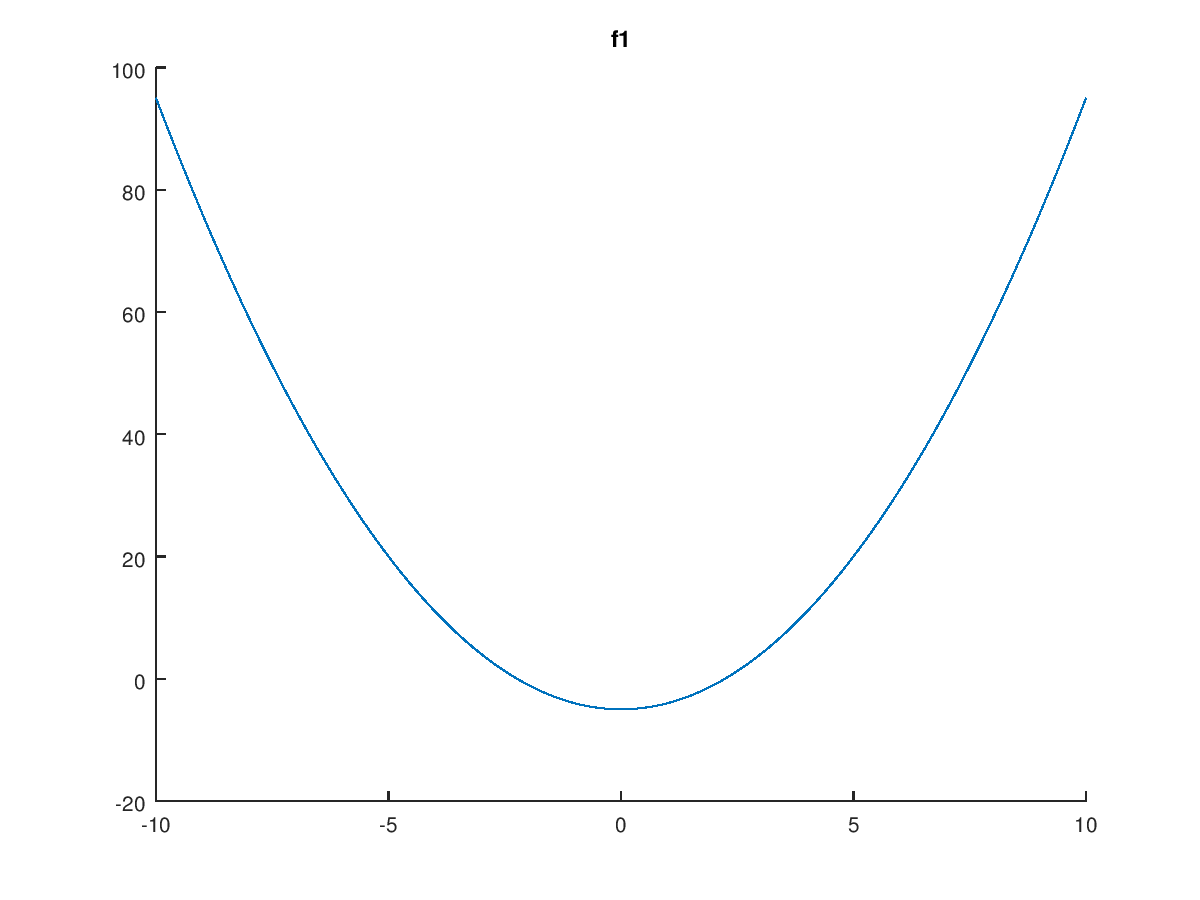
\includegraphics[height=8cm]{f1.png}\\
Figure 1: Shown is function 1 plotted on the interval from [-10,10].\\
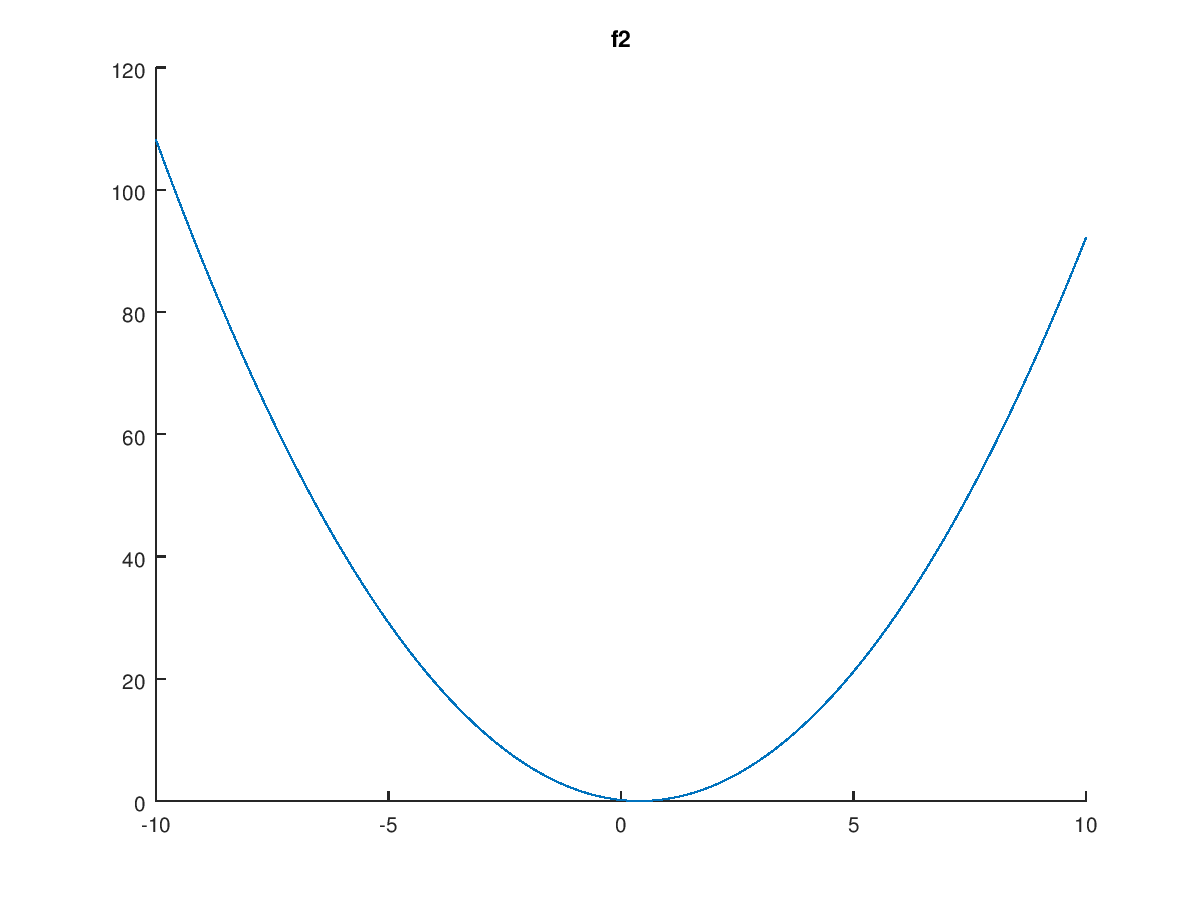
\includegraphics[height=8cm]{f2.png}\\
Figure 2: Shown is function 1 plotted on the interval from [-10,10].\\
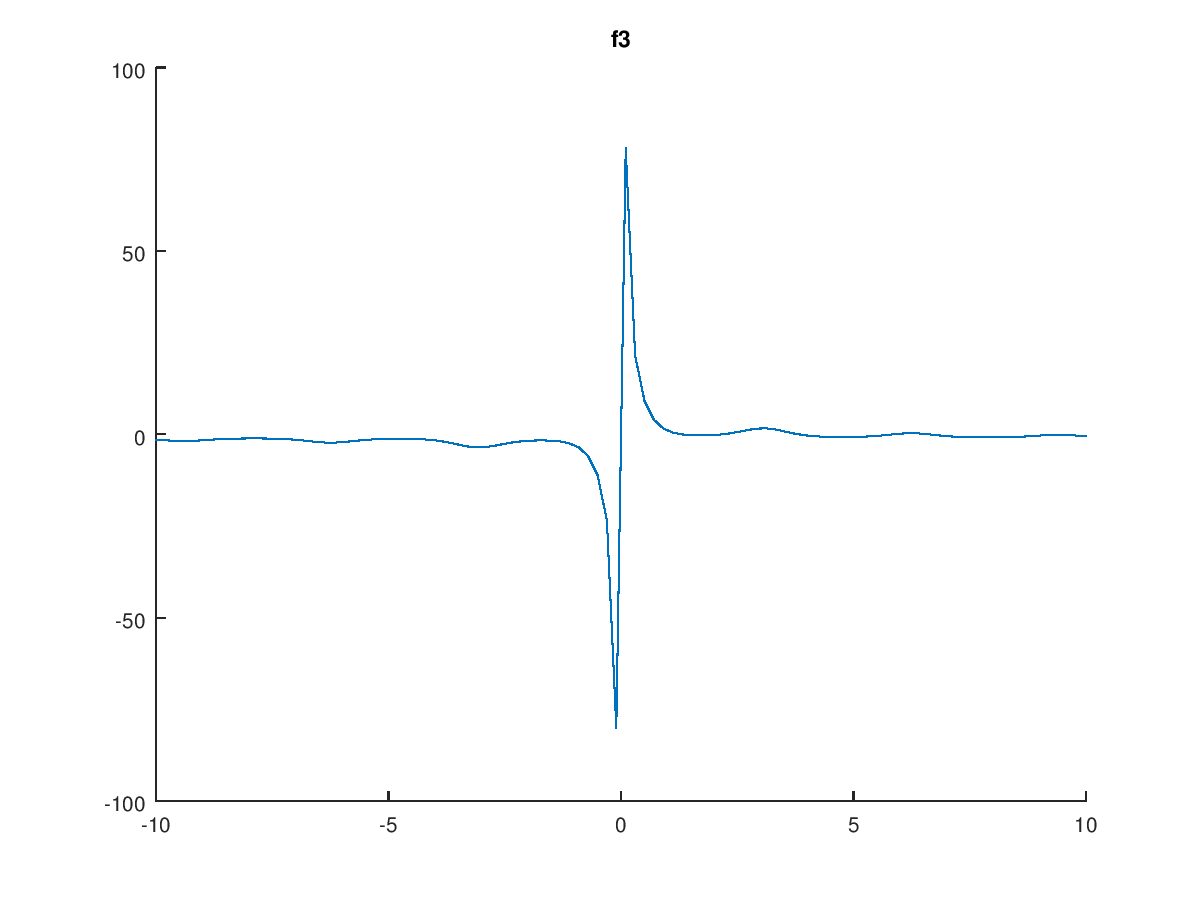
\includegraphics[height=8cm]{f3.png}\\
Figure 3: Shown is function 1 plotted on the interval from [-10,10].\\

The following is the Matlab output after running each method on each function. 
\begin{lstlisting}
-- f1 --
Bisection : Xn 2.2361
Secant : Xn 2.2361
Newtons : Xn 2.2361
-- f2 --
Bisection : Xn 7
Secant : Xn 0.4
Newtons : Xn 0.4
-- f3 --
Bisection : Xn 3.8068
Secant : Xn 2.1981+2.4758e-33i
Newtons : Xn 2.1981	
\end{lstlisting}



\section*{Part B}

\end{document}
